% =====================================================================
% Slide 10: Stage 2 -- LAMMPS framework
% =====================================================================
\begin{frame}{Stage 2: The LAMMPS Framework}
\textbf{LAMMPS}~\citep{thompson2022}\footnote{\tiny LAMMPS = Large-scale Atomic/Molecular Massively Parallel Simulator (Sandia/Temple/NIST).}
is the de-facto MD code in materials science: classical
force-field integration on millions of atoms, MPI + OpenMP +
GPU parallelism, scripted via an in-process Python API.

\medskip
\begin{columns}[T]
\column{0.50\textwidth}
\textbf{Why a custom LAMMPS build was necessary.}
The upstream distribution caps the number of MEAM species at five,
which is incompatible with the 12-element library produced in
Stage~4. The species ceiling was therefore raised to twenty and a
private build of the shared library installed alongside the
standard tooling --- \emph{without this step the entire pipeline
is blocked on the first configuration containing more than five
distinct elements}.

\column{0.49\textwidth}
\begin{block}{Elastic protocol per configuration}
\small
\begin{enumerate}\itemsep0.15em
  \item Build $\sim\!4$\,nm cubic supercell from dominant element's
        lattice and composition-weighted $a_0$.
  \item Stochastically reassign atom types to match the requested
        composition.
  \item Anisotropic minimisation (cell + positions).
  \item Record baseline $\sigma_{xx},\sigma_{yy},\sigma_{zz}$.
  \item Apply $\delta = 10^{-3}$ axial strain
        $(\pm x,\pm y,\pm z)$, re-minimise, record stress.
  \item Central-difference $\to C_{11}\!\times\!3$,
        $C_{12}\!\times\!6$. Voigt average~\citep{voigt}.
\end{enumerate}
\end{block}
\end{columns}
\end{frame}

% =====================================================================
% Slide 11: Stage 2 -- MD results
% =====================================================================
\begin{frame}{Stage 2: MD Results across $\sim\!7800$ Alloys}
\centering
\scriptsize
\begin{tabular}{lrrrrrr}
\toprule
 Quantity   &    N &    Mean &   Median &   Std. &   Min &     Max \\
\midrule
 $E$ (GPa)  & 7815 & 132.88 &  103.61 & 69.10 & 3.07 & 398.31 \\
 $\nu$      & 7815 &   0.319 &    0.326 &  0.063 & 0.011 &   0.497 \\
\bottomrule
\end{tabular}\\[0.1em]
\textit{\scriptsize Dataset statistics after the
$0<E<400$\,GPa, $0<\nu<0.5$ physicality filter.}

\vspace{0.2em}
\begin{columns}[T]
\column{0.50\textwidth}
\centering
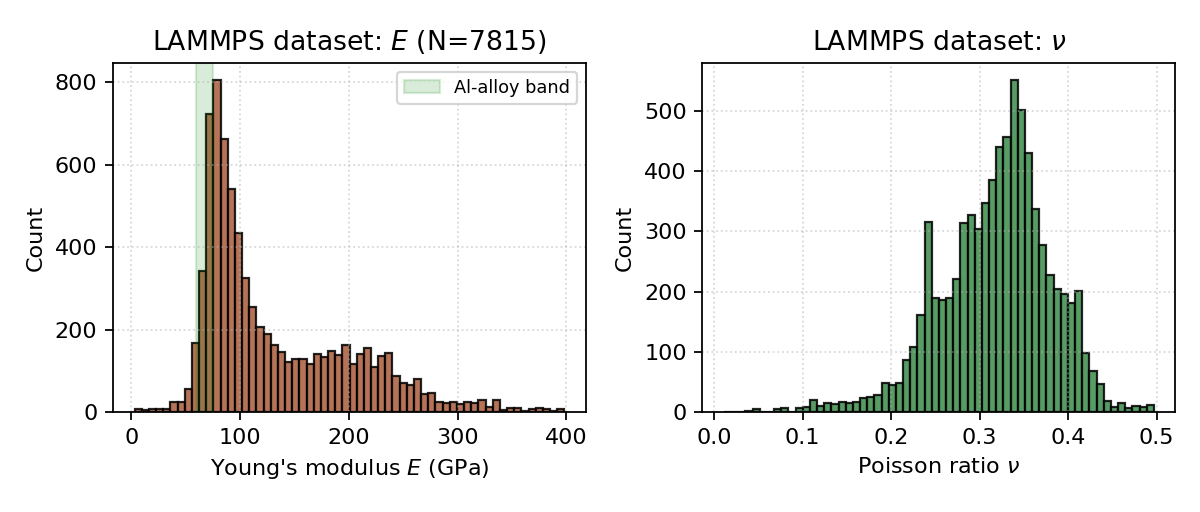
\includegraphics[width=0.99\linewidth]{figures/dataset_distributions.png}\\[-0.2em]
\scriptsize Histograms of $E$ (left) and $\nu$ (right).
Green band marks the $60\!-\!75$\,GPa Al-alloy range.

\column{0.49\textwidth}
\centering
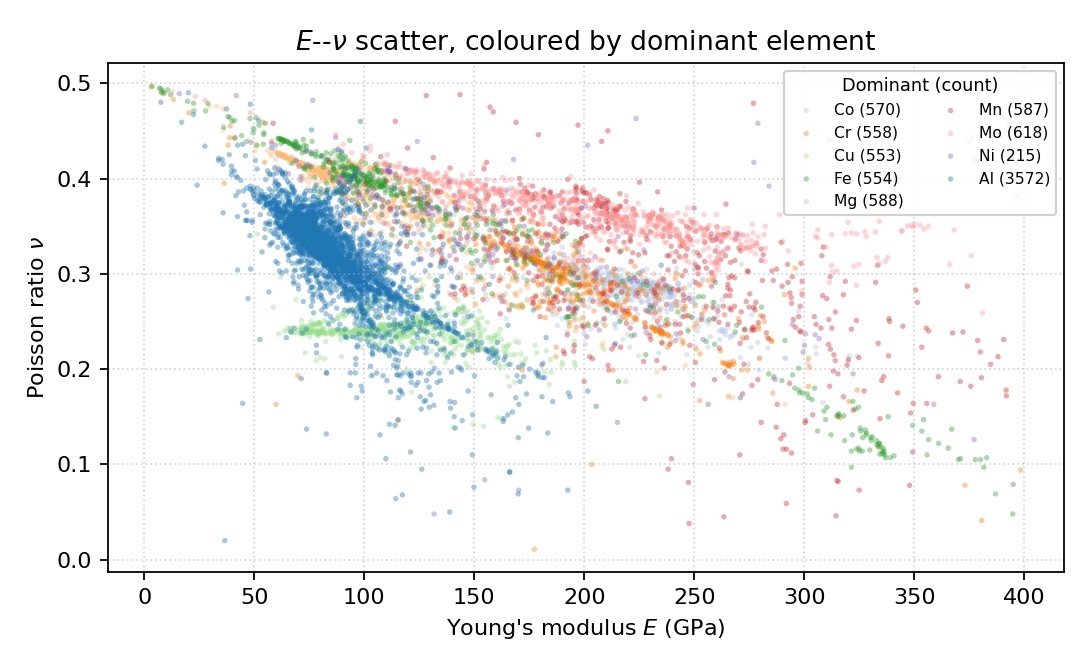
\includegraphics[width=0.92\linewidth]{figures/E_nu_scatter.png}\\[-0.2em]
\scriptsize $E$--$\nu$ scatter coloured by dominant element.
Refractory-rich (Mo, Cr, Fe) populate the high-$E$ wing.
\end{columns}
\end{frame}
